% https://davidstutz.de/illustrating-convolutional-neural-networks-in-latex-with-tikz/

\documentclass[twoside,11pt,a4paper]{article}
 
\usepackage[utf8]{inputenc}
\usepackage{amsmath, amssymb, latexsym}
 
\usepackage{tikz}
 
\usepackage{xcolor}
\definecolor{fc}{HTML}{1E90FF}
\definecolor{h}{HTML}{228B22}
\definecolor{bias}{HTML}{87CEFA}
\definecolor{noise}{HTML}{8B008B}
\definecolor{conv}{HTML}{FFA500}
\definecolor{pool}{HTML}{B22222}
\definecolor{up}{HTML}{B22222}
\definecolor{view}{HTML}{FFFFFF}
\definecolor{bn}{HTML}{FFD700}
\tikzset{fc/.style={black,draw=black,fill=fc,rectangle,minimum height=1cm}}
\tikzset{h/.style={black,draw=black,fill=h,rectangle,minimum height=1cm}}
\tikzset{bias/.style={black,draw=black,fill=bias,rectangle,minimum height=1cm}}
\tikzset{noise/.style={black,draw=black,fill=noise,rectangle,minimum height=1cm}}
\tikzset{conv/.style={black,draw=black,fill=conv,rectangle,minimum height=1cm}}
\tikzset{pool/.style={black,draw=black,fill=pool,rectangle,minimum height=1cm}}
\tikzset{up/.style={black,draw=black,fill=up,rectangle,minimum height=1cm}}
\tikzset{view/.style={black,draw=black,fill=view,rectangle,minimum height=1cm}}
\tikzset{bn/.style={black,draw=black,fill=bn,rectangle,minimum height=1cm}}
 
\begin{document}
 
\begin{figure}[t]
  \centering
  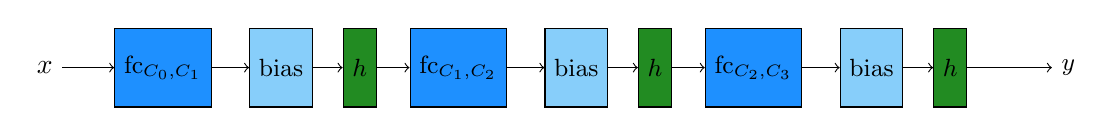
\begin{tikzpicture}
    \node (x) at (0.5,0) {$x$};
    \node[fc] (fc1) at (2,0) {\small$\text{fc}_{C_0, C_1}$};
    \node[bias] (b1) at (3.5,0) {\small$\text{bias}$};
    \node[h] (h1) at (4.5,0) {\small$h$};
    \node[fc] (fc2) at (5.75,0) {\small$\text{fc}_{C_1, C_2}$};
    \node[bias] (b2) at (7.25,0) {\small$\text{bias}$};
    \node[h] (h2) at (8.25,0) {\small$h$};
    \node[fc] (fc3) at (9.5,0) {\small$\text{fc}_{C_2, C_3}$};
    \node[bias] (b3) at (11,0) {\small$\text{bias}$};
    \node[h] (h3) at (12,0) {\small$h$};
    \node (y) at (13.5,0) {\small$y$};
    \draw[->] (x) -- (fc1);
    \draw[->] (fc1) -- (b1);
    \draw[->] (b1) -- (h1);
    \draw[->] (h1) -- (fc2);
    \draw[->] (fc2) -- (b2);
    \draw[->] (b2) -- (h2);
    \draw[->] (h2) -- (fc3);
    \draw[->] (fc3) -- (b3);
    \draw[->] (b3) -- (h3);
    \draw[->] (h3) -- (y);
  \end{tikzpicture}
%  \vskip 6px
  % TODO short caption
  % TODO parameters
  \caption[]{Illustration of a multi-layer perceptron with $L = 3$ fully-connected 
  layers followed by bias layers and non-linearities. The sizes $C_1$ and $C_2$ are
  hyper-parameters while $C_0$ and $C_3$ are determined by the problem at hand.
Overall, the multi-layer perceptron represents a function $y(x;w)$ parameterized by
the weights $w$ in the fully-connected and bias layers.}
  \label{fig:deep-learning-mlp}
\end{figure}
 
\begin{figure}
  \centering
  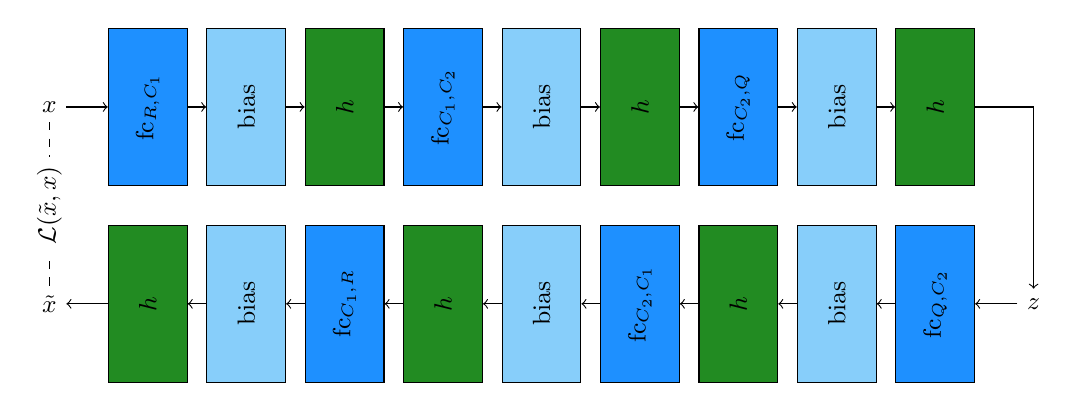
\begin{tikzpicture}
    \node (x) at (1.25,0) {\small$x$};
  
    \node[fc,rotate=90,minimum width=2cm] (fc1) at (2.5,0) {\small$\text{fc}_{R, C_1}$};
    \node[bias,rotate=90,minimum width=2cm] (b1) at (3.75,0) {\small$\text{bias}$};
    \node[h,rotate=90,minimum width=2cm] (h1) at (5,0) {\small$h$};
    \node[fc,rotate=90,minimum width=2cm] (fc2) at (6.25,0) {\small$\text{fc}_{C_1, C_2}$};
    \node[bias,rotate=90,minimum width=2cm] (b2) at (7.5,0) {\small$\text{bias}$};
    \node[h,rotate=90,minimum width=2cm] (h2) at (8.75,0) {\small$h$};
    \node[fc,rotate=90,minimum width=2cm] (fc3) at (10,0) {\small$\text{fc}_{C_2, Q}$};
    \node[bias,rotate=90,minimum width=2cm] (b3) at (11.25,0) {\small$\text{bias}$};
    \node[h,rotate=90,minimum width=2cm] (h3) at (12.5,0) {\small$h$};
  
    \node (z) at (13.75,-2.5) {\small$z$};
  
    \node[h,rotate=90,minimum width=2cm] (h6) at (2.5,-2.5) {\small$h$};
    \node[bias,rotate=90,minimum width=2cm] (b6) at (3.75,-2.5) {\small$\text{bias}$};
    \node[fc,rotate=90,minimum width=2cm] (fc6) at (5,-2.5) {\small$\text{fc}_{C_1, R}$};
    \node[h,rotate=90,minimum width=2cm] (h5) at (6.25,-2.5) {\small$h$};
    \node[bias,rotate=90,minimum width=2cm] (b5) at (7.5,-2.5) {\small$\text{bias}$};
    \node[fc,rotate=90,minimum width=2cm] (fc5) at (8.75,-2.5) {\small$\text{fc}_{C_2, C_1}$};
    \node[h,rotate=90,minimum width=2cm] (h4) at (10,-2.5) {\small$h$};
    \node[bias,rotate=90,minimum width=2cm] (b4) at (11.25,-2.5) {\small$\text{bias}$};
    \node[fc,rotate=90,minimum width=2cm] (fc4) at (12.5,-2.5) {\small$\text{fc}_{Q, C_2}$};
  
    \node (rx) at (1.25,-2.5) {\small$\tilde{x}$};
  
    \draw[->] (x) -- (fc1);
    \draw[->] (fc1) -- (b1);
    \draw[->] (b1) -- (h1);
    \draw[->] (h1) -- (fc2);
    \draw[->] (fc2) -- (b2);
    \draw[->] (b2) -- (h2);
    \draw[->] (h2) -- (fc3);
    \draw[->] (fc3) -- (b3);
    \draw[->] (b3) -- (h3);
    \draw[-] (h3) -- (13.75,0);
    \draw[->] (13.75,0) -- (z);
    \draw[->] (z) -- (fc4);
    \draw[->] (fc4) -- (b4);
    \draw[->] (b4) -- (h4);
    \draw[->] (h4) -- (fc5);
    \draw[->] (fc5) -- (b5);
    \draw[->] (b5) -- (h5);
    \draw[->] (h5) -- (fc6);
    \draw[->] (fc6) -- (b6);
    \draw[->] (b6) -- (h6);
    \draw[->] (h6) -- (rx);
 
    \node[rotate=90] (L) at (1.25, -1.25) {\small$\mathcal{L}(\tilde{x}, x)$};
    \draw[-,dashed] (x) -- (L);
    \draw[-,dashed] (rx) -- (L);
  \end{tikzpicture}
%  \vskip 6px
  \caption{A simple variant of a multi-layer perceptron based auto-encoder.
  Both encoder (top) and decoder (bottom) consist of 3-layer perceptrons
  taking an $R$-dimensional
  input $x$. The parameters $C_1, C_2,$ and $Q$ can be chosen; $Q$ also
  determines the size of the latent code $z$ and is usually chosen significantly
  lower than $R$ such that the auto-encoder learns a dimensionality reduction.
  The non-linearity $h$ is also not fixed and might be determined experimentally.
  The reconstruction loss $\mathcal{L}(\tilde{x}, x)$ quantifies the quality of
  the reconstruction $\tilde{x}$ and is minimized during training.}
  \label{subfig:deep-learning-auto-encoder}
\end{figure}
 
\begin{figure}
  \centering
  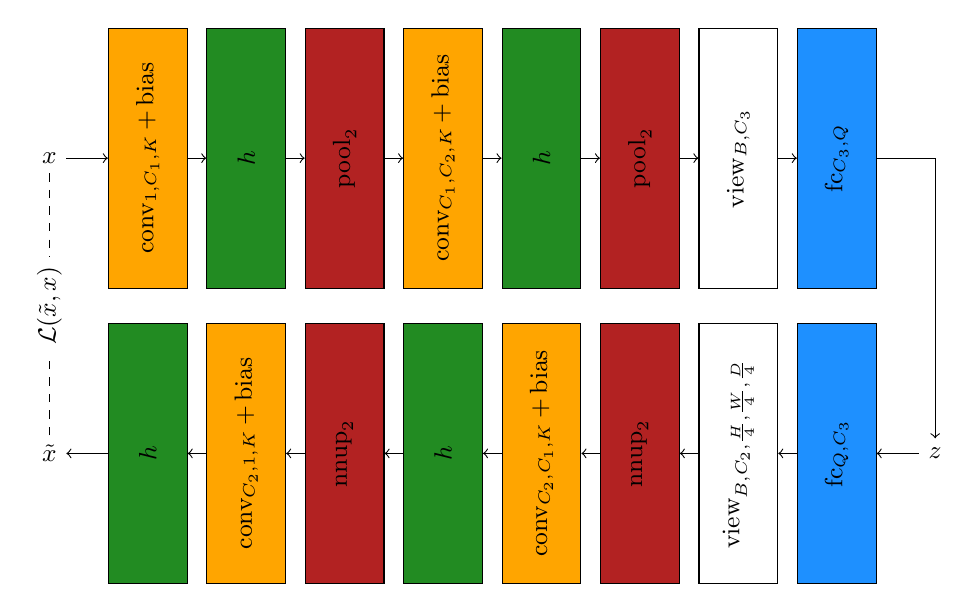
\begin{tikzpicture}
    \node (x) at (1.25,0) {\small$x$};
    
    %\node[noise,rotate=90,minimum width=3.3cm] (noise1) at(1.25,0) {\small$\text{noise}_{\sigma^2}$};
    \node[conv,rotate=90,minimum width=3.3cm] (conv1) at (2.5,0) {\small$\text{conv}_{1, C_1, K}$\,+\,$\text{bias}$};
    %\node[bias,rotate=90,minimum width=3cm] (bias1) at (3.75,0) {$\text{bias}$};
    \node[h,rotate=90,minimum width=3.3cm] (h1) at (3.75,0) {\small$h$};
    \node[pool,rotate=90,minimum width=3.3cm] (pool1) at (5,0) {\small$\text{pool}_{2}$};
    
    \node[conv,rotate=90,minimum width=3.3cm] (conv2) at (6.25,0) {\small$\text{conv}_{C_1, C_2, K}$\,+\,$\text{bias}$};
    %\node[bias,rotate=90,minimum width=3cm] (bias2) at (8.75,0) {$\text{bias}$};
    \node[h,rotate=90,minimum width=3.3cm] (h2) at (7.5,0) {\small$h$};
    \node[pool,rotate=90,minimum width=3.3cm] (pool2) at (8.75,0) {\small$\text{pool}_{2}$};
    \node[view,rotate=90,minimum width=3.3cm] (view2) at (10,0) {\small$\text{view}_{B, C_3}$};
    \node[fc,rotate=90,minimum width=3.3cm] (fc2) at (11.25,0) {\small$\text{fc}_{C_3,Q}$};
    
    \node (z) at (12.5,-3.75) {\small$z$};
    
    \node[h,rotate=90,minimum width=3.3cm] (h4) at (6.25,-3.75) {\small$h$};
    %\node[bias,rotate=90,minimum width=3cm] (bias4) at (8.75,-3.75) {$\text{bias}$};
    \node[conv,rotate=90,minimum width=3.3cm] (conv4) at (7.5,-3.75) {\small$\text{conv}_{C_2, C_1, K}$\,+\,$\text{bias}$};
    \node[up,rotate=90,minimum width=3.3cm] (up4) at (8.75,-3.75) {\small$\text{nnup}_{2}$};
    \node[view,rotate=90,minimum width=3.3cm] (view4) at (10,-3.75) {\small$\text{view}_{B, C_2, \frac{H}{4}, \frac{W}{4}, \frac{D}{4}}$};
    \node[fc,rotate=90,minimum width=3.3cm] (fc4) at (11.25,-3.75) {\small$\text{fc}_{Q,C_3}$};
    
    \node[h,rotate=90,minimum width=3.3cm] (h5) at (2.5,-3.75) {\small$h$};
    %\node[bias,rotate=90,minimum width=3cm] (bias5) at (3.75,-4) {$\text{bias}$};
    \node[conv,rotate=90,minimum width=3.3cm] (conv5) at (3.75,-3.75) {\small$\text{conv}_{C_2, 1, K}$\,+\,$\text{bias}$};
    \node[up,rotate=90,minimum width=3.3cm] (up5) at (5,-3.75) {\small$\text{nnup}_{2}$};
    
    \node (rx) at (1.25,-3.75) {\small$\tilde{x}$};
    
    %\draw[->] (x) -- (noise1);
    \draw[->] (x) -- (conv1);
    \draw[->] (conv1) -- (h1);
    %\draw[->] (bias1) -- (h1);
    \draw[->] (h1) -- (pool1);
    
    \draw[->] (pool1) -- (conv2);
    \draw[->] (conv2) -- (h2);
    %\draw[->] (bias2) -- (h2);
    \draw[->] (h2) -- (pool2);
    \draw[->] (pool2) -- (view2);
    \draw[->] (view2) -- (fc2);
    
    \draw[-] (fc2) -- (12.5,0);
    \draw[->] (12.5,0) -- (z);
    \draw[->] (z) -- (fc4);
    
    \draw[->] (fc4) -- (view4);
    \draw[->] (view4) -- (up4);
    \draw[->] (up4) -- (conv4);
    %\draw[->] (conv4) -- (bias4);
    \draw[->] (conv4) -- (h4);
    
    \draw[->] (h4) -- (up5);
    \draw[->] (up5) -- (conv5);
    \draw[->] (conv5) -- (h5);
    %\draw[->] (bias5) -- (h5);
    \draw[->] (h5) -- (rx);
 
    \node[rotate=90] (L) at (1.25, -1.875) {\small$\mathcal{L}(\tilde{x}, x)$};
    \draw[-,dashed] (x) -- (L);
    \draw[-,dashed] (rx) -- (L);
  \end{tikzpicture}
%  \vskip 6px
  % TODO short caption
  \caption{Illustration of a convolutional auto-encoder consisting of encoder (top)
  and decoder (bottom). Both are modeled using two stages of convolutional
  layers each followed by a bias layer and a non-linearity layer. The encoder uses
  max pooling to decrease the spatial size of the input; the decoder uses upsampling
  to increase it again. The number of channels $C_1$, $C_2$ and $C_3$ as well as
  the size $Q$ are hyper parameters. We assume the input to comprise one channel.
  Again, the reconstruction loss $\mathcal{L}(\tilde{x}, x)$ quantifies the quality of
  the reconstruction and is minimized during training.}
  \label{fig:deep-learning-convolutional-auto-encoder}
\end{figure}
 
\end{document}

